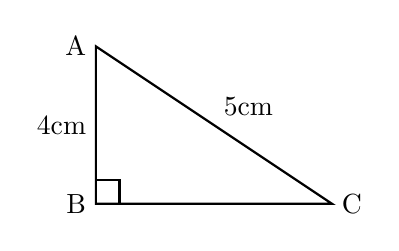
\begin{tikzpicture}[scale=1]

  % Define the vertices of the right-angled triangle
  \coordinate (B) at (0,0);
  \coordinate (C) at (3,0);
  \coordinate (A) at (0,2);

  % Draw the triangle ABC
  \draw[thick] (A) -- (B) -- (C) -- cycle;

  % Draw the right-angle symbol at B
  \draw[thick] (0.3,0) -- (0.3,0.3) -- (0,0.3);

  % Add labels for the vertices
  \node[left] at (A) {A};
  \node[left] at (B) {B};
  \node[right] at (C) {C};

  % Add labels for the side lengths
  \node[left] at (0,1) {4cm};
  \node[above right] at (1.5,1) {5cm};

\end{tikzpicture}